\chapter{K-indukciós algoritmus szoftverellenőrzésre}

Ebben a fejezetben bemutatom azokat a technológiákat, melyek szükségesek a programom technikai oldalának megértéséhez. Először ismertetem a Control Flow Automata ábrázolás részleteit (Alfejezet \ref{sec:control_flow_automata})), aztán az előző fejezetben bemutatott jelölésrendszerrel formalizálom az algoritmust (Alfejezet \ref{sec:formalizalt_alg}).

\section{Control Flow Automata}
\label{sec:control_flow_automata}

A programkódokat sokféleképpen ábrázolhatjuk \cite{soft_ver_akos}. Legismertebb a programkód, melyet az ember könnyen, gyorsan tud olvasni illetve írni, ellenben a bájtkóddal, melyet a számítógép tud jóval hatékonyabban kezelni. A szoftveres modellellenőrzés elvégzéséhez a programkódot matematikailag pontos, formális ábrázolásban kell megadni, melyet a számítógép is jól tud kezelni. Egy széleskörűen ismert és használt ábrázolásmód a \emph{Control Flow Automaton} (CFA), mely egy gráf alapú ábrázolást biztosít a programokhoz. 

\paragraph{Szintaxis.}
A CFA  formálisan egy $\mathit{CFA} = (V, H, I_0, E)$ négyes \cite{beyer13}, ahol

\begin{itemize}
	\item $V = \{v_1, v_2, \ldots\}$ a változók halmaza. Mindegyik $v_i \in V$ változó rendelkezik egy $D_{v_i}$ doménnel, mely megszabja, hogy $v_i$ milyen értékeket vehet fel,
	\item \emph{H} a helyek halmaza,
	\item $I_0 \in H$ a kezdőállapota a gráfnak, a program belépőpontját mutatja,
	\item $E \subseteq H \times \mathit{Op} \times H$ az irányított élek halmaza, melyek helyeket kötnek össze és a változókra vonatkozó utasításokkal vannak felcímkézve
\end{itemize}

% TODO: operator vagy utasitas

\paragraph{Utasítások.}
Háromféle utasítással foglalkozunk: 

\begin{itemize}
	\item A \emph{hozzárendelés} utasítás a $v_i := \mathit{expr}$ összefüggéssel írható le. Azt jelöli, hogy a baloldali $v_i$ változóhoz hozzárendeljük a jobb oldali kifejezést. Fontos, hogy az $\mathit{expr}$ kifejezésnek is ugyanolyan doménnel kell rendelkeznie, mint a $v_i \in V$ változónak.
	
	\item A \emph{feltevés} operátor a $[\mathit{cond}]$ formában írható le, ahol $\mathit{cond}$ egy bináris (\emph{Boolean}) kifejezés (feltétel). Ha egy él rendelkezik $\mathit{[cond]}$ feltétellel, akkor abban az esetben csakis akkor sülhet el (kerülünk át az egyik helyről a másikra), ha a feltétel teljesül. A feltétel változón nem változtat, arra nem hat ki.
	
	\item A \emph{havoc} operátor a $\mathit{havoc}~v_i$ formában írható le, ahol $v_i \in V$ egy változó. A \emph{havoc} hozzá rendel a $v_i$ változóhoz egy nem-determinisztikus értéket, a többi változót érintetlenül hagyja. Például arra lehet használni, mikor szimulálni szeretnénk a felhasználói bemenetet.
\end{itemize}

\paragraph{Grafikai megjelenítés.}
A helyeket körök, az éleket nyilak jelölik. Az egyes élek felett illetve mellett láthatóak az utasítások, amely jelen esetben hozzárendelés vagy feltevés. A kezdőállapotot egy bejövő nyíllal jelöljük. \cite{soft_ver_akos}.

\begin{figure}[!htb]
	\begin{subfigure}[b]{.30\linewidth}
		\begin{lstlisting}
	int x = 1;
	if (y <= 10) {
			y = 10;
	} else {
			while (x < y) {
					x = 2 * x;
					y = y - 1;
			}
	}
	x = y + 1; \end{lstlisting}
	\caption{Egyszerű C program.}
	\label{fig:cfa1}		
	\end{subfigure}	
\hfill
\begin{subfigure}[b]{.63\linewidth}
	\centering
	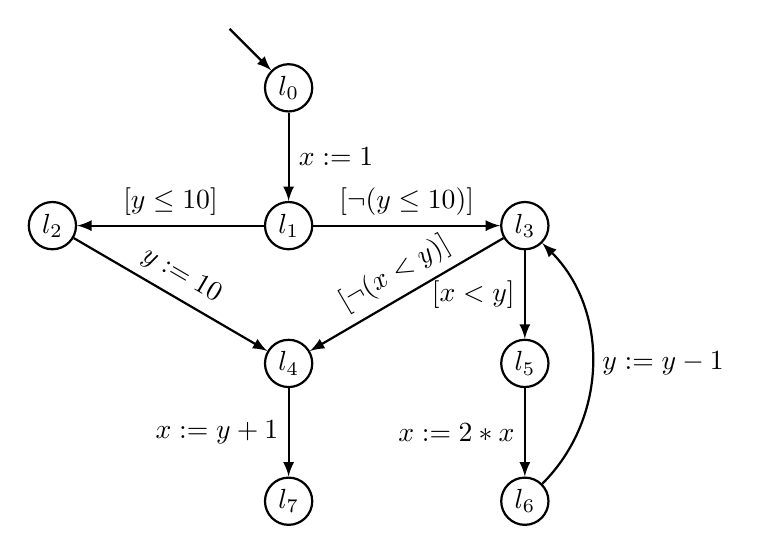
\begin{tikzpicture}
		\tikzstyle{loc}=[circle,align=center,draw,fill=white,thick,minimum size=0.6cm,inner sep=2]
		\tikzstyle{edge}=[-latex,thick]
		
		\node [loc] (l0) at (0, 0) {$l_0$};
		\draw[edge] (-0.75, 0.75)--(l0);
		
		\node [loc] (l1) at ( 0, -1.75) {$l_1$};
		\node [loc] (l2) at (-3, -1.75) {$l_2$};
		\node [loc] (l3) at ( 3, -1.75) {$l_3$};
		\node [loc] (l4) at ( 0, -3.5)  {$l_4$};
		\node [loc] (l5) at ( 3, -3.5)  {$l_5$};
		\node [loc] (l6) at ( 3, -5.25) {$l_6$};
		\node [loc] (l7) at ( 0, -5.25) {$l_7$};
		
		\draw[edge] (l0) -- node[midway, right]{$x := 1$}  (l1);
		\draw[edge] (l1) -- node[midway, above, sloped]{$[y \leq 10]$}  (l2);
		\draw[edge] (l1) -- node[midway, above, sloped]{$[\neg(y \leq 10)]$}  (l3);
		\draw[edge] (l2) -- node[midway, above, sloped]{$y := 10$}  (l4);
		\draw[edge] (l3) -- node[midway, above, sloped]{$[\neg(x < y)]$}  (l4);
		\draw[edge] (l3) -- node[midway, left]{$[x < y]$}  (l5);
		\draw[edge] (l4) -- node[midway, left]{$x := y+1$} (l7);
		\draw[edge] (l5) -- node[midway, left]{$x := 2*x$} (l6);
		\draw[edge] (l6) to [bend right = 45] node[midway, right]{$y := y-1$} (l3);
	\end{tikzpicture}
	\caption{A program CFA ábrázolása.}
	\label{fig:cfa2}
\end{subfigure}
\caption{Egy C program és a hozzá tartozó Control Flow Automaton (CFA).}
\label{fig:cfa}
\end{figure}

\begin{example}
	Egy C nyelvű program és egy hozzá tartozó CFA látható a \ref{fig:cfa} ábrán. A kezdőhely az $l_0$, a termináló hely az $l_7$, mely lehet végső- (final location) illetve hibahely (error location). Egy útvonal a kezdőhelytől az $l_4$ helyre leírható úgy, hogy $l_0 \rightarrow l_1 \rightarrow l_2 \rightarrow l_4$. Az $l_1$ helyen egy elágazást figyelhetünk meg, ahol ha feltétel a $[y \leq 10]$ teljesül, akkor úgy a program az $l_1$ helyről továbbmegy az $l_2$ helyre, míg ha nem teljesül, akkor az $l_3$ helyre kerül a program. Az elágazásokban a kimenő élekre a feltételek úgy vannak megfogalmazva, hogy míg az egyiken az eredeti feltétel, addig a másikon annak a negáltja figyelhető meg. Ez azért van így, hogy szemléltesse az ábra, hogy ezt egy algoritmus fogja feldolgozni, amely számára ebben a formátumban könnyebb megadni az automatát.
\end{example}

\paragraph{Programábrázolás.} A \ref{fig:structprog} ábra megmutatja, hogy az alap elemei a strukturált programozásnak miként képezhetőek le CFA alakba \cite{soft_ver_akos}.
\begin{itemize}
	\item \emph{Szekvenciális} állításokat (\ref{fig:structprogseq} és \ref{fig:structprogseqcfa} ábra) úttal reprezentáljuk, mely helyek és élek közt alternál.
	
	\item \emph{Feltételes elágazásokat} (pl. \textit{ha-akkor} állítások, \ref{fig:structprogsel} és \ref{fig:structprogselcfa} ábra) különváló utakkal tudunk reprezentálni őrfeltételekkel.
	
	\item \emph{Feltételes ciklusokat} (\ref{fig:structprogrep} és \ref{fig:structprogrepcfa} ábra) a CFA-ban körökkel tudunk ábrázolni. Egy vezérlési hely felel a ciklusfejért, amelyből két kimenő él fut. Az egyik bemegy a ciklusba, a másik pedig kilép abból. A ciklusban további szekvenciák, elágazások vagy akár újabb ciklusok is történhetnek, azonban az út mindig visszatér a ciklusfejhez.
\end{itemize}

\begin{figure}[!htb]
	\begin{subfigure}[b]{.29\linewidth}
		\begin{lstlisting}
			stmt1;
			stmt2;
			...\end{lstlisting}
		\caption{Szekvencia a programban.}
		\label{fig:structprogseq}		
	\end{subfigure}	
	\hfill
	\begin{subfigure}[b]{.29\linewidth}
		\begin{lstlisting}
			if (cond) {
				stmt1;
				...
			} else {
				stmt2;
				...
			}\end{lstlisting}
		\caption{Feltételes elágazás a programban.}
		\label{fig:structprogsel}		
	\end{subfigure}	
	\hfill
	\begin{subfigure}[b]{.29\linewidth}
		\begin{lstlisting}
			while (cond) {
				stmt;
				...
			}\end{lstlisting}
		\caption{Feltételes ciklus a programban.}
		\label{fig:structprogrep}		
	\end{subfigure}	
	\hfill
	\begin{subfigure}[b]{.3\linewidth}
		\centering
		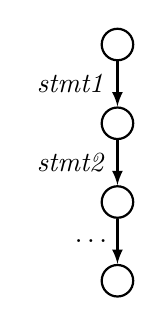
\begin{tikzpicture}
			\tikzstyle{loc}=[circle,draw,fill=white,thick,minimum size=0.4cm,inner sep=0]
			\tikzstyle{edge}=[-latex,thick]
			
			\node [loc] (l0) at ( 0, 0) {};
			\node [loc] (l1) at ( 0,-1) {};
			\node [loc] (l2) at ( 0,-2) {};
			\node [loc] (l3) at ( 0,-3) {};
			
			\draw[edge] (l0)--node[left]{$\mathit{stmt1}$}(l1);
			\draw[edge] (l1)--node[left]{$\mathit{stmt2}$}(l2);
			\draw[edge] (l2)--node[left]{$\ldots$}(l3);
		\end{tikzpicture}
		\caption{Szekvencia a CFA-ban.}
		\label{fig:structprogseqcfa}
	\end{subfigure}
	\hfill
	\begin{subfigure}[b]{.3\linewidth}
		\centering
		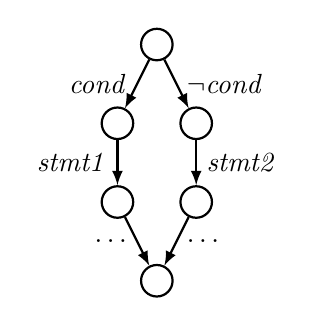
\begin{tikzpicture}
			\tikzstyle{loc}=[circle,draw,fill=white,thick,minimum size=0.4cm,inner sep=0]
			\tikzstyle{edge}=[-latex,thick]
			
			\node [loc] (l0) at (   0, 0) {};
			\node [loc] (l1) at (-0.5,-1) {};
			\node [loc] (l2) at ( 0.5,-1) {};
			\node [loc] (l3) at (-0.5,-2) {};
			\node [loc] (l4) at ( 0.5,-2) {};
			\node [loc] (l5) at (   0,-3) {};
			
			\draw[edge] (l0)--node[left]{$\assumeop{\mathit{cond}}$}(l1);
			\draw[edge] (l0)--node[right]{$\assumeop{\neg \mathit{cond}}$}(l2);
			\draw[edge] (l1)--node[left]{$\mathit{stmt1}$}(l3);
			\draw[edge] (l2)--node[right]{$\mathit{stmt2}$}(l4);
			\draw[edge] (l3)--node[left]{$\ldots$}(l5);
			\draw[edge] (l4)--node[right]{$\ldots$}(l5);
		\end{tikzpicture}
		\caption{Feltételes elágazás a CFA-ban.}
		\label{fig:structprogselcfa}
	\end{subfigure}
	\hfill
	\begin{subfigure}[b]{.3\linewidth}
		\centering
		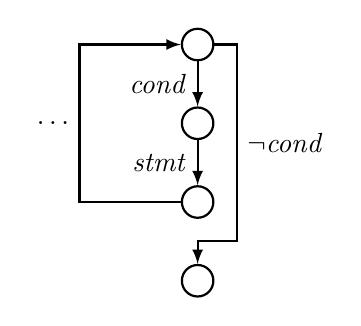
\begin{tikzpicture}
			\tikzstyle{loc}=[circle,draw,fill=white,thick,minimum size=0.4cm,inner sep=0]
			\tikzstyle{edge}=[-latex,thick]
			
			\node [loc] (l0) at ( 0, 0) {};
			\node [loc] (l1) at ( 0,-1) {};
			\node [loc] (l2) at ( 0,-2) {};
			\node [loc] (l3) at ( 0,-3) {};
			
			\draw[edge] (l0)--node[left]{$\assumeop{\mathit{cond}}$}(l1);
			\draw[edge] (l1)--node[left]{$\mathit{stmt}$}(l2);
			\draw[edge] (l2)--(-1.5,-2)--node[left]{$\ldots$}(-1.5,0)--(l0);
			\draw[edge] (l0)--(0.5,0)--node[right]{$\assumeop{\neg \mathit{cond}}$}(0.5,-2.5)--(0,-2.5)--(l3);
		\end{tikzpicture}
		\caption{Feltételes ciklus a CFA-ban.}
		\label{fig:structprogrepcfa}
	\end{subfigure}
	\caption{A strukturált programozás elemei (szekvencia, feltételes elágazás, feltételes ciklus) és a megvalósításuk CFA modelleken.}
	\label{fig:structprog}
\end{figure}

\section{A formalizált algoritmus}
\label{sec:formalizalt_alg}

A fenti ismeretek segítségével hogy tudnánk belátni, hogy a modell a \emph{P} tulajdonságra nézve biztonságos?

Például úgy, ha megnézzük, hogy tetszőleges nemnegatív \emph{i} egész esetén teljesül-e a
\begin{align}
	\forall s_{0} \dots s_{i}:~\neg(I(s_{0}) \wedge utvonal(s_{[0..i]}) \wedge \neg P(s_{i}))
\end{align}
feltétel. Ha megsérül valamelyik elérhető állapotban, akkor ezzel a módszerrel meg fogjuk találni és az oda vezető útvonal ellenpélda lesz a modell \emph{P}-biztonságosságára. Ez egy elvárható eredmény: az algoritmusnak két féle kimenetele kell, hogy legyen: vagy az, hogy a modell \emph{P}-tulajdonságra nézve biztonságos (minden elérhető állapot teljesíti), vagy az, hogy a modell nem \emph{P}-biztonságos, ekkor egy ellenpéldát is kell adnia, mely bizonyítja, hogy az adott kezdőállapotból elindulva, azon végighaladva valóban egy hibaállapotba kerülünk.

Ha a rendszer \emph{P}-biztonságos, akkor (TODO) minden \emph{i}-re igaz lesz, hiszen nem fogunk tudni találni olyan \emph{i} értéket, melyre ne teljesülne. Felvetődhet a kérdés, hogy mikortól lehet azt mondani, hogy \emph{i} további növelése céltalan, mert már teljes bizonyossággal kijelenthetjük, hogy a modell \emph{P}-biztonságos? A $I(s_{0}) \wedge utvonal(s_{[0..i]})$ feltétel önmagában nem fog gyorsítást eredményezni: vagy végig megy az állapottéren amilyen hosszan csak lehetséges (ezt szeretnénk lerövidíteni), tekintve, hogy minden állapotnak van egy szülőállapota a \emph{T} tranzakciós reláción keresztül, vagy végtelen ciklusba kerül.

Ennél jobb stratégia, ha akkor állunk meg, mikor $I(s_{0})~\wedge~ cmUtvonal(s_{[0..i]})$ ellentmondásos lesz. Ezt használva addig folytatjuk a keresést, míg az összes, ciklusmentes útvonalat be nem jártuk. Legrosszabb esetben ekkor is végigmegy a program a teljes állapottéren, viszont ha az állapottérben ciklikusság figyelhető meg, akkor azt a stratégia maximálisan kihasználja: nem fog végtelen ciklusba kerülni, illetve átlagosan rövidebb (de bizonyosan nem hosszabb) útvonalakat fog bejárni, mint az $I(s_{0}) \wedge utvonal(s_{[0..i]})$.

Ehhez hasonlóan tehetjük azt is, hogy addig ellenőrzünk, amíg a $cmUtvonal(s_{[0..i]}) \wedge \neg P(s_{i})$ nem lesz ellentmondásos: egy, a \emph{P} tulajdonságot sértő állapotból (hibaállapotból) kiindulva addig megyünk ciklusmentes útvonalakon visszafelé, míg be nem járjuk a teljes állapotteret (ez esetben kijelenthetjük, hogy a rendszer nem-\emph{P}-biztonságos), ellenben ha nem járunk be minden \emph{elérhető} állapotot, akkor a rendszer \emph{P}-biztonságos (feltéve, hogy egyik hibaállapotból sem tudjuk bejárni a teljes rendszert). Ez azzal magyarázható, hogy ha a kezdőállapotok halmaza nem elérhető a hibaállapotokból (mert visszafele haladva útközben elakadunk), akkor kijelenthetjük, hogy a modell biztonságos.
\newline
\newline
A \emph{k}-indukció alapú szoftververifikáció az előbb elmondottakra épül. A módszer lényege, hogy elindulunk mind a kezdőállapotokból, mind a hibaállapotokból: míg az előbbiekből előrefelé, addig az utóbbiakból visszafelé. Kijelenthető, hogy a modell biztonságos, ha az előrefelé haladó keresés bejárta a teljes elérhető állapotteret (nincs több ciklusmentes útvonal)\footnote{Természetesen ha közben hibaállapotba jutna, akkor a teljes modellellenőrzés megakadna, s így nem tudná bejárni a teljes állapotteret.}, illetve akkor is biztonságos, ha a hátrafelé haladó keresés megakad.

A \ref{sec:k_induction}.-as fejezetben bemutatott, és így a módszer nevét adó \emph{k-indukció} úgy kerül a képbe, hogy ha a modellt bejárjuk \emph{k} mélységig, és belátjuk a fentebb említett metodika alapján, hogy a modell biztonságos, akkor kijelenthető, hogy $k+1$ mélységre is biztonságos lesz \cite{donaldson_cikk}, illetve mellé az is, hogy ezzel az indukciós lépést bizonyítottuk \cite{k_induction_article}:

\begin{comment}
\begin{algorithm}[H]
\SetAlgoLined
\KwResult{}
i=0\\
\While{True}{
instructions\\
\eIf{condition}{
instructions1\\
instructions2\\
}{
instructions3\\
}
}
\caption{Checking if model is \emph{P}-safe}
\end{algorithm}í
\end{comment}